\documentclass[kulak]{kulakarticle} % options: kulak (default) or kul

\usepackage[dutch]{babel}
\usepackage{graphicx}

\title{Analyseren van een wetenschappelijk artikel}
\author{Vincent Van Schependom}
\date{Academiejaar 2023 -- 2024}
\address{
	\textbf{Groep Wetenschap \& Technologie Kulak} \\
	Informatica \\
	Wetenschappelijk Schrijven}

\begin{document}

\maketitle

\noindent Analyse van de tekst Cyclist Fall Detection System via the Internet of Things (IoT) \cite{KitTamJun2023CFDS}.

\subsection*{Plannen}

\textbf{Hoe dragen de illustraties bij tot een beter begrip van de tekst?}

\noindent In de tekst worden, gemiddeld genomen, 1 of 2 illustraties per pagina gebruikt. Deze illustraties zijn meestal flowcharts of grafieken, maar de tekst bevat ook minder relevante illustraties, zoals afbeeldingen van de sensoren.  De flowcharts helpen de lezer bij het begrijpen van het denkproces achter de technologie. De grafieken geven de opgemeten data uit het onderzoek weer, om zo bepaalde verbanden duidelijk te maken. Dankzij deze grafieken is er bijvoorbeeld een duidelijk link zichtbaar tussen de metingen van de versnellingsmeter en het ogenblik waarop beslist wordt om hulp in te schakelen.

\subsection*{Ontwerpen}

\textbf{Kan de lezer op basis van de titel de inhoud van het artikel correct inschatten?}

\noindent Het is voor de lezer na het lezen van de titel meteen duidelijk waarover het gaat. We weten dat het gaat over een crashdetectiesysteem en dat bovendien IoT aan bod zal komen in de tekst.

\subsection*{Schrijven}

\textbf{Belemmeren formules en symbolen de leesbaarheid van de tekst?}

\noindent Zoals te zien is in figuur \ref{fig:formules}, worden in de tekst een aantal formules genummerd. Er wordt echter nergens in de tekst naar deze nummering verwezen. Deze overbodige nummering kan dus weggelaten worden om de leesbaarheid van de tekst te bevorderen.

\subsection*{Opmaken}

\textbf{Hoe onderscheiden de sectieniveaus zich van de platte tekst?}

\noindent De auteurs gebruiken vette tekst in hoofdletters voor de titels in het artikel. Voor de subtitels gebruiken de auteurs schuingedrukte tekst. De hoofdstuktitel van het hoofdstuk met de methodiek staat bijvoorbeeld in vette hoofdletters, terwijl elke subtitel van dit hoofdstuk schuingedrukt staat.

\subsection*{Reviseren}

\textbf{Geef enkele voorbeelden van de tweeledige structuur in de tekst.}

\noindent In de inleiding wordt het onderzoek gesitueerd en worden de doelstellingen geformuleerd. Doorheen het artikel wordt er dan dieper ingegaan op de manier waarop de doelstellingen uit de inleiding concreet bereikt kunnen worden.  Bovendien worden de titels en subtitels van elk hoofdstuk eerst verklaard en gesitueerd alvorens er dieper op elk onderwerp wordt ingegaan.

Bij het hoofdstuk over \textit{Location Services} wordt bijvoorbeeld eerst uitgelegd wat \textit{location services} precies zijn, alvorens men uitlegt hoe deze aan bod kwamen in het onderzoek.

\newpage

\begin{figure}
	\centering
	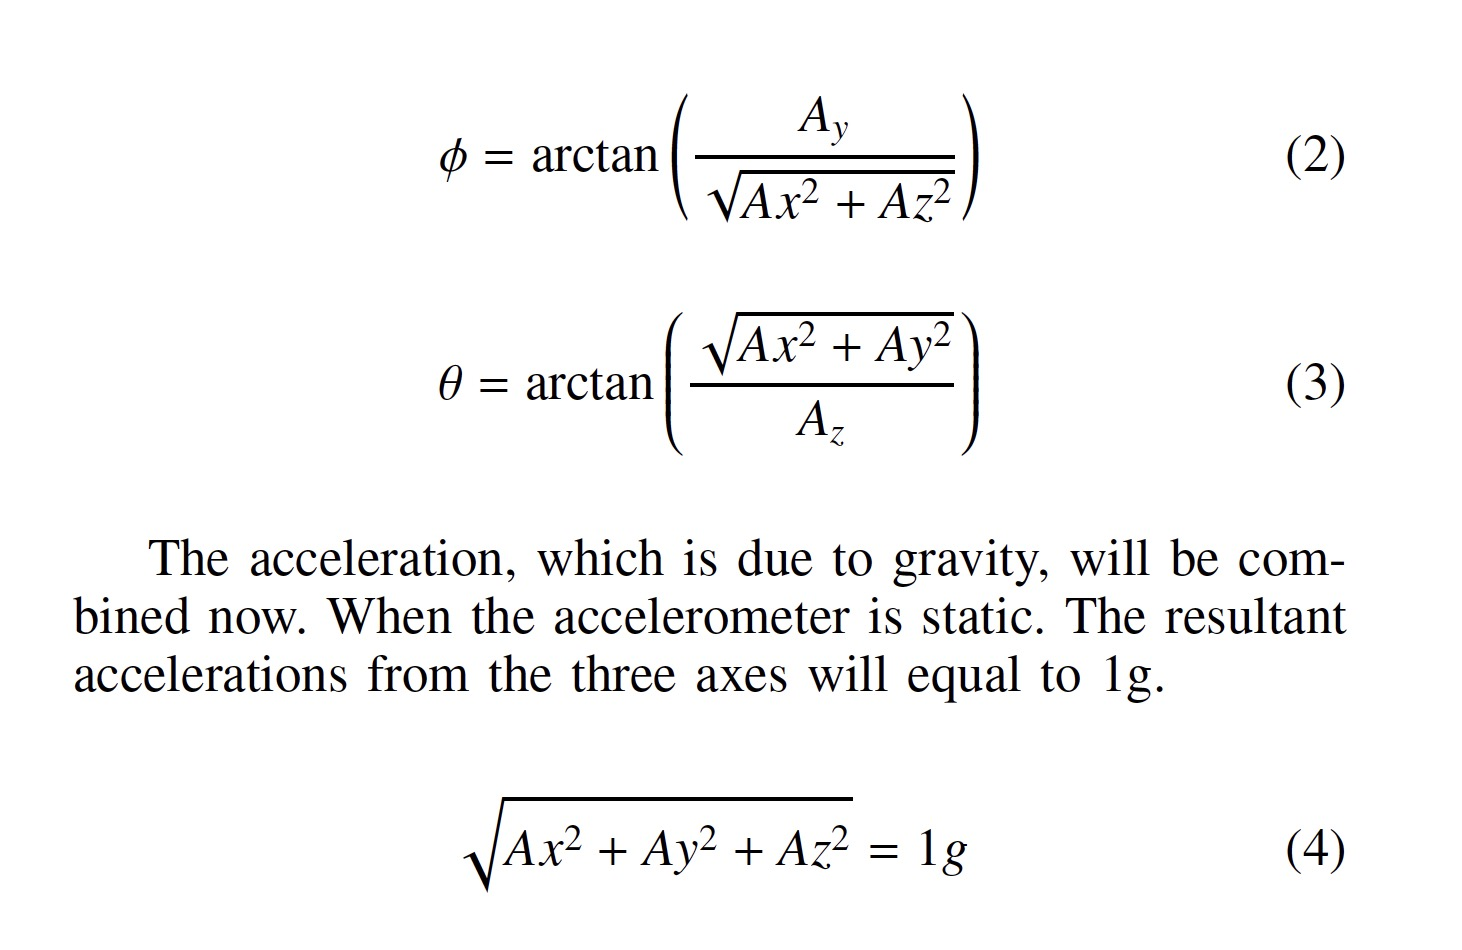
\includegraphics[width= 0.7\textwidth]{formules}
	\caption{Een schermafbeeldling uit het geanalyseerde artikel. De formules hebben een nummering, waarnaar nooit verwezen wordt en die bijgevolg weggelaten kan worden.}
	\label{fig:formules}
\end{figure}

\bibliographystyle{unsrt}
\bibliography{bibliografie}

\end{document}
